\section{Einleitung}
\label{s:intro}


%%%%%%%%%%%%%%%%%%%%%%%%%%%%%%%%%%%%%%%%%%%%%%%%%%%%%%%%%%%%%%
\subsection{Ein Abschnitt der Einleitung}
\label{ss:intro:abc}

\section{Technische Grundlagen und Implementierungen}
\label{s:grundlagen}

Im folgenden Kapitel wird ein Überblick über die zentralsten \ac{ble} Anwendungen gegeben. Zusätzlich wird die Hardwareebene im Bezug auf die physikalischen Voraussetzungen und die genutzten Frequenzbereiche näher betrachtet. 

\subsection{Beispiele für Implementierungen}
\label{ss:grundlagen:beispiele}

Im einundzwanzigsten Jahrhundert steigt die Verwendung von Geräten, welche drahtlos mit einem Empfangsgerät kommunizieren können. Vor allem die Einführung des Smartphones hat an diesem Punkt die drahtlose Kommunikation vorangetrieben. Nutzer wollen viele Funktionen zur Verfügung gestellt bekommen, um den persönlichen Alltag einfacher gestalten zu können.\\

\noindent Schon vor der Einführung des Smartphones war das Kommunikationsprotokoll "`Bluetooth"' auf Mobiltelefonen verfügbar. Dabei wurde es hauptsächlich zum Datentransfer zwischen zwei Bluetoothfähigen Endgeräten verwendet. Das Hauptproblem, welches der Nutzer dabei erfahren musste, ist, dass diese Form der Datenübertragung sehr viel Zeit in Anspruch genommen hat. Dies lässt sich auf die geringe Datenmenge zurückführen, die pro Paket möglich ist.\\

\noindent Nachdem das Smartphone immer mehr an Beliebtheit gewonnen hat und sich der Begriff des \ac{iot} entwickelt hat, reagierte die Bluetooth \ac{sig}, indem sie ein Protokoll erarbeiteten, welches einen möglichst geringen Stromverbrauch, eine geringe Bandbreite und niedrige Komplexität bietet \cite[Seite 1]{Townsend14:GSB}.\\

\noindent Mit der Einführung von \ac{ble} kam die Möglichkeit kleine Datensignale zwischen Geräten auszutauschen. Ein aktuell sehr bekanntes Beispiel sind dabei sogenannte "`Smartwatches"'. Diese bieten neben der Möglichkeit die Uhrzeit bereitzustellen viele weitere Funktionen, wie beispielsweise die Steuerung von Telefongesprächen, oder die Fernsteuerung der Musikwiedergabe. Der Nutzer erhält durch ein derartiges Gerät die Möglichkeit, sein Smartphone in gewissen Bereichen fernzusteuern.\\

\noindent Beinahe jeder Mensch in der heutigen Zeit besitzt und nutzt ein Smartphone. Jedes Smartphone ist dabei mit einer Bluetoothschnittstelle ausgestattet. Dieser Sachverhalt liefert die Möglichkeit, nicht nur eine "`Smartwatch"' mit dem Smartphone zu verbinden, sondern jegliches Empfangsgerät, welches der Nutzer benötigen könnte. Besonders beliebt sind dabei Fitnessgeräte, die dem Nutzer Informationen über sein Fitnesslevel liefern.\\

\noindent Allerdings liefert der Sachverhalt, dass beinahe jeder Nutzer Bluetooth nutzt auch andere "`Usecases"'. Mit sogenannten "`Beacons"' (siehe Kapitel \ref{s:ibeacon}) kann man beispielsweise mit einem Smartphone Informationen von einem oder mehreren "`Beacons"' erfassen und in einer App oder im Browser gesammelt aufbereitet anzeigen. Ein "`Beacon"' ist ein \ac{ble} Gerät, welches ausschließlich Informationen sendet. So kann man beispielsweise in einem Raum mit mehreren solchen Geräten stehen und Informationen über verschiedene Lebensmittel, oder deren Preise erhalten. Mit dieser Möglichkeit kann ein Nutzer noch besser und zielgerichteter mit sachdienlichen Informationen versorgt werden.\\

\noindent Sollte man die Absicht haben, ein eigenes Gerät zu entwickeln, welches mittels \ac{ble} kommuniziert, gibt es mehrere Anbieter für Hardwarekomponenten für verschiedene Anwendungsfälle. Besonders nennenswert sind dabei die Firmen "`Nordic"' und "`Texas Instruments"'.\\

\noindent Die Firma "`Nordic"', welche Kompononenten für verschiedenste Kommunikationsprotokolle anbietet, ist Mitglied bei der Bluetooth \ac{sig} und hat einen signifikanten Beitrag zum fortschritt von \ac{ble} beigetragen. Sie war auch eine der ersten Firmen, die günstige \ac{ble} Komponenten auf den Markt gebracht haben \cite[Seite 75]{Townsend14:GSB}.\\

\noindent Die Firma "`Texas Instruments"' hingegen war als erstes dazu in der Lage, ein \ac{ble} fähiges Peripheriegerät auf den Markt zu bringen. Zusätzlich ist "`Texas Instruments"' als einiger Anbieter "`Feature complete"'. Das heißt, dass die Geräte den kompletten Funktionsumfang des \ac{ble} Stacks anbieten \cite[Seite 79]{Townsend14:GSB}.\\ 

\subsection{Hardware}
\label{ss:grundlagen:hardware}

Auf Hardwareebene gibt es verschiedenste Ansätze, um ein \ac{ble} Modul zu entwickeln. Die bekanntesten Firmen, welche derartige Geräte produzieren sind unter anderem "`Texas Instruments"' und "`Nordic"'. Allerdings gibt es noch viele weitere Firmen mit eigenen \ac{ble} Chips. Aus diesem Grund gibt es keine einheitliche Hardware, die alle diese Chips verwenden. Die einzige Anforderung, welche diese Chips erfüllen müssen ist, dass sie nach den \ac{ble} Standards handeln müssen, welche die Bluetooth \ac{sig} vorgibt. Im folgenden werden nun einige markante Eigenschaften beschrieben, welche \ac{ble} auf Hardwareebene interessant machen.\\

\noindent Betrachtet man beispielsweise den Kostenfaktor, so fällt auf, dass es hier eine große Preisspanne für verschiedenste Module gibt. Einfache Module, welche sich für die Programmierung mit der Arduino Entwicklungsumgebung eignen sind schon für unter 10€ verfügbar. Andere Geräte, welche einen höheren industriellen Standard erfüllen können wiederum mehr als 30€ kosten. Allerdings ist ein \ac{ble} Modul selten wirklich teuer. Der niedrige Preis von derartigen Geräten ist daher einer der Gründer für den großen Erfolg von \ac{ble} und das beinahe jedes Smartphone ein entsprechendes Modul besitzt hilft hier sicherlich auch enorm.\\

\noindent Wenn man über drahtlose Kommunikation spricht ist ein Aspekt von besonderer Wichtigkeit. Die Reichweite, die das jeweilige Protokoll in der Lage ist zu erreichen. Im Fall von \ac{ble} sind drei Leistungsklassen definiert, anhand derer festgelegt wird, wie groß die Reichweite ist. Die meistgenutzte Klasse ist dabei die 3. Klasse, die eine Reichweite von 10 Metern erreicht. Diese hat die geringste Sendeleistung und kann auch maximal eine Wand durchdringen. Mit absteigender Klasse erhöht sich die Sendeleistung und die Reichweite. Das hat zur Folge, dass Geräte mit Sendeklasse eins bis zu 100 Meter Reichweite erreichen können. Der Energieverbrauch dieser Geräte ist jedoch um ein vielfaches höher als in Klasse drei. Wo Klasse drei mit einem Milliwatt sendet, sendet Klasse eins mit 100 Milliwatt. Da \ac{ble} jedoch großen Wert auf niedrigen Energieverbrauch legt, wird fast ausschließlich die dritte Klasse verwendet. Geräte mit unterschiedlichen Klassen können auch miteinander kommunizieren. Jedoch wird immer die Klasse für die Kommunikation gewählt, welche beide Kommunikationspartner bereit sind einzugehen. Wenn man also ein Gerät hat, welches mit Klasse eins senden möchte und ein weiteres mit Klasse drei, dann wird die gesamte Kommunikation in Klasse drei abgehalten \cite[Seite 411]{Sauter18:GMK}.\\ 

\subsection{Frequenzbereich}
\label{ss:grundlagen:frequenz}

Da \ac{ble} ein Teil des Bluetoothstacks ist, sind die physikalischen Eigenschaften, die sowohl hinter Bluetooth Klassik, als auch \ac{ble} stecken identisch. Der Frequenzbereich, indem Bluetooth sendet ist dementsprechend auch der selbe. Allerdings gibt es einen Unterschied, was die Kanäle angeht, in denen gesendet wird.\\

\noindent Der Frequenzbereich in dem sich Bluetooth bewegt liegt zwischen 2,4GHz und 2,4835GHz auf dem \ac{ism} Band \cite[Seite 16]{Townsend14:GSB}. Diesen Bereich teilt sich Bluetooth mit einigen anderen Kommunikationsprotokollen, weshalb es zwischen den Protokollen zu Kollisionen bei der Übertragung kommen kann. Aus diesem Grund teilt Bluetooth seinen Bereich in mehrere Kanäle auf. Bei Bluetooth Klassik ist der Frequenzbereich in insgesamt 79 Kanäle unterteilt \cite[Seite 410]{Sauter18:GMK}. \ac{ble} teilt den Bereich allerdings nur in 40 Kanäle auf \cite[Seite 16]{Townsend14:GSB}. Daraus resultiert, dass die Kanäle bei \ac{ble} doppelt so groß sind wie bei Bluetooth Klassik. Der Grund für diese Kanalunterteilung ist das sogenannte "`Frequency Hopping"', welches unter Kapitel \ref{sss:funktionsweise:physical} näher betrachtet wird.\\  

\section{Funktionsweise Bluetooth Low Energy}
\label{s:funktionsweise}
beispielsweise
Im nachfolgenden Kapitel wird nun auf die Softwareseitigen Aspekte des \ac{ble} Stacks eingegangen. Dabei finden die Architektur und die Kommunikation besondere Beachtung. Zusätzlich wird ein Überblick geboten, welche Möglichkeiten diese Technologie dem Nutzer bietet.\\  

\subsection{Protokollstack}
\label{ss:funktionsweise:protokollstack}

In Abbildung \ref{FIG:protokollstack} ist der Protokollstack von \ac{ble} zu sehen. Dabei sind die drei Ebenen "`Controller"', "`Host"' und "`Application"' zu erkennen. Auf der untersten Ebene liegt der "`Controller"', in welchem das "`Physical Layer"' und das "`Linked Layer"' enthalten sind. Zwischen "`Host und "`Controller"' liegt das sogenannte \ac{hci}, welches die Schnittstelle zwischen den beiden Kommunikationspartnern darstellt. Im "`Host"' wiederum befinden sich sämtliche Protokolle und Profile, die notwendig sind, um Kommunikation zu ermöglichen. An der Spitze des Protokollstacks befindet sich die "`Applikation"' in der die Logik und Nutzerschnittstelle des aktuellen Anwendungsfalls liegt \cite[15]{Townsend14:GSB}. Wie diese einzelnen Komponenten funktionieren und untereinander kommunizieren ist in den nachfolgenden Abschnitten erläutert.\\  
 
\begin{figure}[h]
\centering
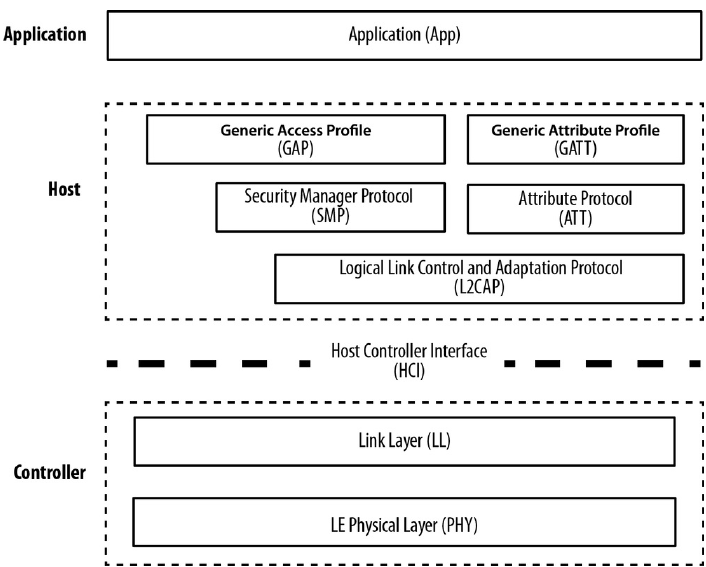
\includegraphics[width=\linewidth]{\figdir/BLE_Protokolstack}
\caption{\ac{ble} Protokollstack \cite[Seite 16]{Townsend14:GSB}}
\label{FIG:protokollstack}
\end{figure}

\subsubsection{Physical Layer}
\label{sss:funktionsweise:physical}

Das sogenannte "`Physical Layer"' bildet die Basis der Kommunikation bei einer Großzahl von Gerätearchitekturen. In dieser Schicht werden digitale Signale, also Bitfolgen, in analoge Signale umgewandelt. Dieser Vorgang wird zum Senden von Nachrichten über eine physikalische Schnittstelle benötigt. Die Rückübersetzung in eine digitale Bitfolge wird ebenfalls im "`Physical Layer"' erledigt \cite[Seite 16]{Townsend14:GSB}. Als physikalisches Medium bieten sich dabei eine Vielzahl von Möglichkeiten, wie unter anderem Magnetismus, Strom, oder Licht \cite[Seite 95 - 101]{Tanenbaum14:CN}.\\

\noindent Bei \ac{ble} ist die besagte physikalische Schnittstelle die Luft. \ac{ble} nutzt in dieser wie in Kapitel \ref{ss:grundlagen:frequenz} erläutert einen definierten Frequenzbereich um Nachrichten zu übertragen. Dabei belegt \ac{ble} nur einen sehr kleinen Bereich des verfügbaren Spektrums. Insgesamt deckt der verfügbare Frequenzbereich in etwa einen Bereich von 30.000GHz ab. In ihm werden unter anderem Radiowellen, Fernsehübertragungen, Satellitensignale und viele weitere Nachrichtenpakete transportiert \cite[Seite 107]{Tanenbaum14:CN}. Im Frequenzbereich in dem \ac{ble} übertragen wird befinden sich trotz des großen Spektrums einige konkurrierende Technologien, wie beispielsweise "`Wireless LAN"' \cite[Seite 17]{Townsend14:GSB}. Aus diesem Grund verwendet Bluetooth im allgemeinen das sogenannte "`Frequency Hopping Spread Spectrum"'. Dafür wird der verfügbare Frequenzbereich im Fall von \ac{ble} in 40 Kanäle aufgeteilt. Von diesen werden die letzten drei Kanäle zum "`Advertisment"', also zur Bekanntmachung, verwendet. Über diese gibt sich ein Gerät zu erkennen, welches bereit zum Verbinden ist. Ein suchendes Gerät wiederum überprüft ausschließlich diese drei Kanäle nach verfügbaren Geräten. Die restlichen 37 Kanäle werden anschließend für die Übertragung verwendet. Dabei wird zu Beginn des Datenaustausches eine Sprungfrequenz vereinbart, welche daher für jede neue Verbindung voneinander abweicht. Nachdem die Verbindungsinformationen vereinbart wurden, beginnt der Datenaustausch. In Formel \ref{eq:ble:frequencyhopping} ist zu erkennen, wie die Verbindungspartner gegenseitig abstimmen, in welchen Kanal sie als nächstes wechseln werden. Diese Berechnung führt jedes Gerät unter Berücksichtigung der vereinbarten Verbindungsinformationen selbst aus \cite[Seite 17]{Townsend14:GSB}. 
\begin{equation}
\label{eq:ble:frequencyhopping}
Kanal = (aktueller Kanal + Sprungfrequenz) \mod 37
\end{equation}
Sollte dennoch ein Paket bei der Übertragung verloren gehen, wird dieses nach sofortigem Kanalwechsel erneut übertragen. Sollte es mehrfach zu Problemen mit einem oder mehreren Kanälen kommen führt Bluetooth eine Kanalabschätzung durch. Dabei wird eine "`Channel Bitmap"' mit Kanälen erzeugt, welche eine hohe Interferenz aufweisen. Diese werden anschließend für die laufende Verbindung gesperrt. Um festzulegen, ob ein Kanal blockiert ist, gibt es die folgenden drei Möglichkeiten:

\begin{itemize}
	\item[1.]{\ac{rssi}}
	\item[2.]{Eine hohe Packetfehlerrate}
	\item[3.]{Informationen eines Endgerätes mit Zugriff auf konkurrierende Funktechnologien}
\end{itemize}       

\noindent Welche dieser Optionen verwendet wird ist allerdings vom Standard nicht vorgeschrieben und kann deshalb selbstständig definiert werden \cite[Seite 411]{Sauter18:GMK}.\\

\noindent 

\subsubsection{Linked Layer}
\label{sss:funktionsweise:linked}

Das "`Linked Layer"' liegt in der Architektur direkt auf dem "`Physical Layer"'. Dabei stellt es entweder die zu sendenden Daten bereit, oder verarbeitet die vom "'Physical Layer"' empfangenen. Um dies bewerkstelligen zu können, werden Nachrichten nach einem definierten Schema in sogenannte "`Frames"' gepackt. Diese enthalten zusätzlich zur eigentlichen Nachricht wichtige Informationen bezüglich des Paketes. Mit diesen kann unter anderem überprüft werden, ob es zu Fehlern bei der Übertragung gekommen ist, indem man eine "`CRC Checksumme"' bildet \cite[Seite 194]{Tanenbaum14:CN}.\\

\noindent Das "`Linked Layer"' wird bezüglich der zu verarbeitenden Daten für jede Kommunikationsart angepasst. Im Fall von \ac{ble} gibt es daher einige Eigenschaften, welche sich von anderen Protokollen unterscheiden. Zum einen gilt es zu beachten, dass die \ac{ble} Kommunikation auf einem Nachrichtenaustausch beruht, der sehr schmale Zeitfenster aufweist in denen Nachrichten gesendet werden können. Aus diesem Grund wird das "`Linked Layer"' hier weitestgehend von den oberen Protokollschichten getrennt und kommuniziert nur über das \ac{hci} mit diesen. Daraus Folgt wiederum, dass das "`Linked Layer"' sehr schnell in der Verarbeitung von Daten ist \cite[Seite 17f]{Townsend14:GSB}.\\

\noindent Jedes \ac{ble} Gerät verfügt über eine eindeutige Adresse. Diese ist Aufgebaut wie eine "`MAC Adresse"'. Diese Adresse kann das Gerät bei einem "`Advertisement"' versuch broadcasten und andere Geräte können sich dann mit dieser Koppeln. Der Verbindungsprozess hat also verschiedene Rollenverteilungen die von der auszuführenden Aktion des Gerätes abhängen. So ist ein Gerät, welches auf einen Verbindungspartner wartet, ein "`Advertiser"'. Das bedeutet, dass dieses Gerät dauerhaft auf den Advertisementkanälen seine Adresse und andere wichtige Informationen für einen potentiellen Verbindungspartner preisgibt. Der potentielle Verbindungspartner in diesem Fall hat die Rolle des "`Scanners"' inne. Das bedeutet, dass er gerne eine Verbindung eingehen würde. Um dies zu tun überprüft er die drei Advertisementkanäle nach "`Advertisern"'. Diese werden dann beispielsweise dem Nutzer in einer Liste angezeigt. Hier werden nur Geräte angezeigt, welche noch keine aktive Verbindung aufweisen. Das liegt daran, dass die Verbindungspartner bei einer erfolgten Verbindung ihre Rollen ändern. Der "`Scanner"' wird zum "`Master"' der Verbindung und steuert diese. Der "`Advertiser"' wiederum wird zum "`Slave"' der Verbindung und folgt den Anweisungen des "`Masters"' bezüglich des Timings. In der Regel handelt es sich bei "`Slave"' Geräten um einfache Geräte mit niedrigen Funktionalitäten, wohingegen der "`Master"' meist ein leistungsstärkeres Gerät darstellt \cite[Seite 18f]{Townsend14:GSB}.\\  

\noindent Bei \ac{ble} tritt gegenüber dem normalen Bluetoothprotokoll die Besonderheit auf, dass es nicht zwangsläufig zu einer Verbindung zwischen "`Master"' und "`Slave"' kommen muss. Geräte wie "`Beacons"' beispielsweise arbeiten nur auf den Advertisementkanälen und senden dauerhaft Informationen an alle \ac{ble} Geräte in Reichweite \cite[Seite 13]{Gast14:BPA}. Näheres hierzu findet sich unter Kapitel \ref{s:ibeacon}.\\


\noindent Wenn ein Gerät auf der Suche nach einem Verbindungspartner ist, hat es zwei Möglichkeiten. Zum einen kann es einen passiven Scan auf die Advertisementkanäle durchführen, bei dem der "`Advertiser"' nicht mitbekommt, dass er erfasst wurde. Zum anderen kann ein aktiver Scan durchgeführt werden, mit dem eine aktive Anfrage an das zur Verfügung stehende Gerät gesendet wird, um weitere Informationen einzuholen und das Gerät über einen potentiellen Verbindungspartner zu informieren. Die Nachricht, welche bei einem aktiven Scan an den "`Scanner"' gesendet wird enthält drei zentrale Informationen:
\begin{itemize}
	\item[1.]{Die Möglichkeit einer Verbindung (Ja/Nein)}
	\item[2.]{Die Möglichkeit einen aktiven Scan durchführen zu können (Ja/Nein)}
	\item[3.]{Die Information, ob der "`Advertiser"' ein "`Broadcaster"' ist (Ja/Nein)}
\end{itemize}           
Sollte der "`Advertiser"' ein "`Broadcaster"' sein ist es erlaubt, nutzerspezifische Daten in den Nachrichten auszutauschen. In allen anderen Fällen werden hier ausschließlich verbindungsspezifische Daten ausgetauscht \cite[Seite 20f]{Townsend14:GSB}.\\

\noindent Für den Fall, dass der "`Advertiser"' kein "`Broadcaster"' ist, ergibt sich die Möglichkeit eine Verbindung aufzubauen. Um das zu bewerkstelligen sendet der "`Scanner"' eine Verbindungsanfrage. Eine Verbindung in \ac{ble} steht für eine Abfolge von Verbindungsevents, bei denen Nachrichten ausgetauscht werden. Der "`Scanner"' nimmt nun die Rolle des "`Masters"' an und legt in der Verbindungsanfrage drei grundlegende Eckpunkte fest. Zum einen die Zeitspanne, die vergeht, bis ein neues Verbindungsevent stattfindet. Je größer diese Zeitspanne ist, desto weniger Energie wird verbraucht. Ein weiterer Punkt ist die Anzahl der Verbindungsevents, welche der "`Slave"' überspringen darf, ohne die Verbindung zu beenden. Der letzte Punkt ist die Zeit, die vergehen darf, bis ein Timeout ausgelöst wird \cite[Seite 21f]{Townsend14:GSB}.\\ 

\noindent Im "`Linked Layer"' wird die maximale Paketgröße festgelegt. In älteren Versionen von \ac{ble} lag die Payloadgröße, welche jedes Nachrichtenpaket maximal beinhalten konnte, bei 27 Byte. In Abbildung \ref{FIG:payload} ist der Aufbau eines Nachrichtenpaketes dargestellt. Besonders wichtig ist hierbei die Größe der Payload. Bezüglich dieser kann man erkennen, dass sich diese mit Version 4.2 auf 251 Bytes erhöht hat. Das wurde durch die Einführung der "`Data Length Extension"' ermöglicht. Dieses Upgrade schafft die Voraussetzungen dafür, Nachrichten in weniger Zeit übertragen zu können, da mehr Informationen in ein Paket passen \cite{Gupta:WWW}.\\   

\begin{figure}[h]
	\centering
	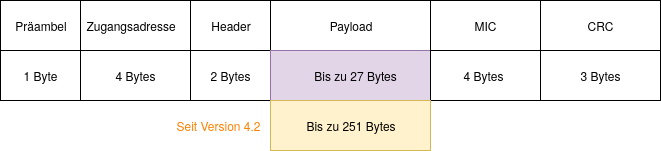
\includegraphics[width=\linewidth]{\figdir/Payload}
	\caption{Aufbau eines Nachrichtenpaketes bei \ac{ble}}
	\label{FIG:payload}
\end{figure}

\noindent Sollte ein Paket fehlerhaft übertragen werden, wird dieses mittels der CRC Checksumme entdeckt und dieses Paket wird so lange wiederholt, bis die Checksumme korrekt ist. Dabei gibt es keine Obergrenze für die Anzahl an Wiederholungen \cite[Seite 23]{Townsend14:GSB}.\\

\subsubsection{Protokolle}
\label{sss:funktionsweise:protocoll}

In Abbildung \ref{FIG:protokollstack} ist zu erkennen, dass sich zwischen den Schichten des "`Controllers"' und des tatsächlichen "`Hosts"' das \ac{hci} befindet. Dessen Zweck zeigt sich hauptsächlich bei leistungsstarken Geräten. Diese bieten den Vorteil, dass komplexe Funktionen ausgeführt werden können. Da \ac{ble} allerdings einige Funktionalitäten aufweist, welche für die Kommunikation essenziell sind und möglichst schnell abgehandelt werden müssen, werden diese zumeist in einen separaten Hardwarechip ausgelagert. Somit liegt der "`Controller"' Teil des Protokollstacks in der Regel nicht auf dem Prozessor. Die eigene Implementierung und die dafür benötigten Protokollschichten liegen allerdings aufgrund der Leistung auf der CPU. Einzige Ausnahme davon sind kleine Geräte, welche nicht viel Leistung benötigen und nur einfache Funktionen mit \ac{ble} ausführen. Bei diesen kann es sehr wohl vorkommen, dass der komplette Protokollstack auf einem einzigen Hardwarechip lokalisiert ist \cite[Seite 24]{Townsend14:GSB}. Im Folgenden wird nun erläutert welche Schichten sich im "'Host"' befinden und es wird auf deren Funktionen eingegangen.\\  

\noindent Die Basis der Protokoll bietet das \ac{l2cap}. Dessen Hauptaufgabe ist es, zu gewährleisten, dass die Pakete, welche von den höheren Schichten versendet werden wollen, den Kriterien der "`Controller"' Schichten entsprechen. Ebenfalls verarbeitet es die empfangenen Pakete der unteren Schichten. Dabei liegt das Hauptaugenmerk auf der Fragmentierung der Pakete in die entsprechenden Pakete. Wie unter Abschnitt \ref{sss:funktionsweise:linked} erläutert kann \ac{ble} nur eine begrenze Anzahl an Bytes pro Paket versenden. Das \ac{l2cap} sorgt dafür, dass Nachrichten entsprechen aufgeteilt an das Linked Layer übergeben werden \cite{TI:WWW}.\\

\begin{figure}[h]
	\centering
	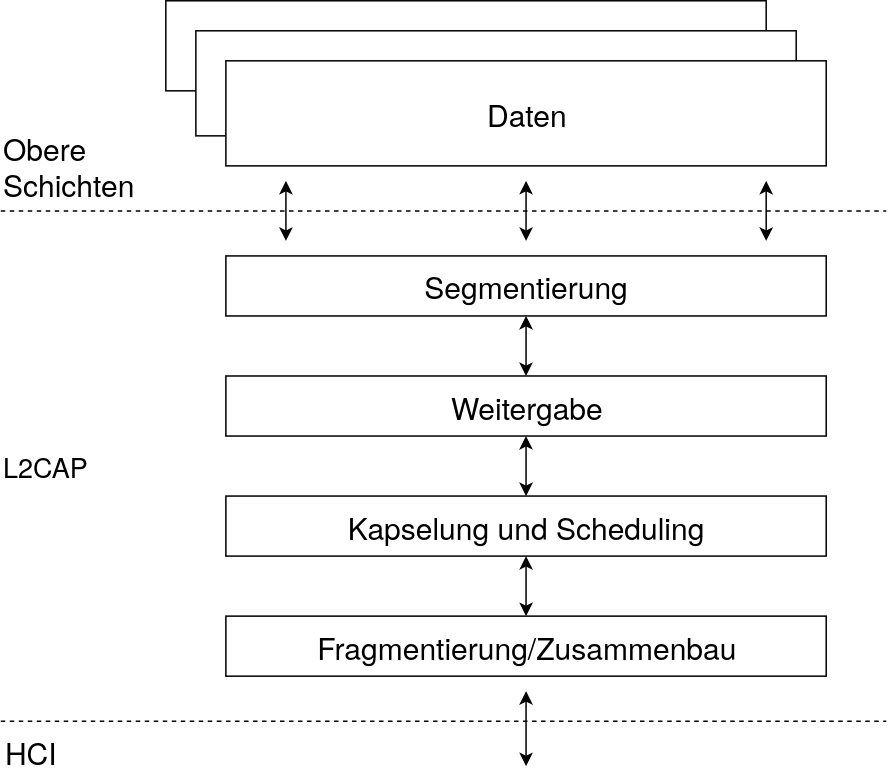
\includegraphics[width=0.5\linewidth]{\figdir/L2CAP}
	\caption{Funktionsebenen des \ac{l2cap} \cite{TI:WWW}}
	\label{FIG:l2cap}
\end{figure}

\noindent Zusätzlich fungiert das \ac{l2cap} als Protokoll Multiplexer. Das bedeutet, dass es mehrere Schichten über sich akzeptiert und diese in das Standard \ac{ble} Paketformat bringt \cite[Seite 25]{Townsend14:GSB}. In Abbildung \ref{FIG:l2cap} sind die einzelnen Arbeitsschritte und deren Zusammenhang dargestellt. Daraus geht hervor, dass jedes Datenpaket vier Bereiche durchlaufen muss, um von den oberen Schichten in das \ac{hci} zu gelangen. In die andere Richtung werden die selben Ebenen durchlaufen. Dementsprechend werden hier Pakete segmentiert, bevor sie von der Flusskontrolle des \ac{l2cap} an die Kapselung und den "`Scheduler"' weitergereicht werden. Dieser gibt die aufgeteilten Pakete dann nach und nach in die Fragmentierung weiter, in welcher die Nachricht in Pakete geteilt wird, die den \ac{ble} Standards entsprechen. Hier wird auch der "`Payload"' Teil der Paketstruktur angelegt, welche in Abbildung \ref{FIG:payload} dargestellt ist. Die maximale Größe des Paketes, welche durch die Fragmentierung laufen kann nennt sich \ac{mtu}. In Abbildung \ref{FIG:mtu} ist zu erkennen, wie die Fragmentierung funktioniert. Dabei wird ein Header definiert, der die notwendigen Informationen enthält, welche der Empfänger benötigt. Die restlichen Pakete werden dann gesendet und auf Empfängerseite wieder anhand der Headerinformationen zusammengesetzt. Die maximale Größe einer \ac{mtu} wird von Client und Server festgelegt. Dabei sendet der Client seine maximal unterstützte \ac{mtu} Größe und erfragt die serverseitige. Nachdem diese Informationen ausgetauscht sind, wird die \ac{mtu} auf die niedrigere Größe der Verbindungspartner gesetzt \cite{TI:WWW}.\\ 

\begin{figure}[h]
	\centering
	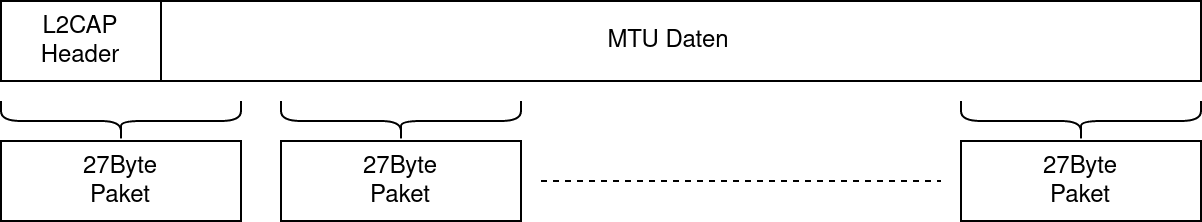
\includegraphics[width=0.75\linewidth]{\figdir/MTU}
	\caption{Fragmentierung der \ac{mtu} \cite{TI:WWW}}
	\label{FIG:mtu}
\end{figure}

\noindent Auf der nächsten Ebene des Protokollstacks befinden sich wie in Abbildung \ref{FIG:protokollstack} zu sehen die beiden Protokolle \ac{smt} und \ac{att}.\\

\noindent Bei \ac{ble} Geräten handelt es sich immer um Server, Client, oder beides. Das \ac{att} ist ein zustandsloses Client/Server Protokoll, welches Schnittstellen für die Kommunikation zwischen den jeweiligen Verbindungspartnern gewährleistet. Dabei kann maximal eine Anfrage parallel durchgeführt werden. Sollte also eine Anfrage länger benötigen, können keine weiteren Anfragen gesendet werden, bis die Schnittstelle wieder frei ist \cite[Seite 26]{Townsend14:GSB}.\\

\noindent Auf Serverseite sind sogenannte Attribute hinterlegt. Diese enthalten einen Wert, der bei Zugriff auf dieses Attribut gelesen, oder überschrieben werden kann. Der Zugriff auf ein Attribut benötigt eine entsprechende Berechtigung. Sollte diese erfüllt sein, kann man über einen 16 Bit "`Handle"' oder einen \ac{uuid} auf die Ressource zugreifen. Neben den klassischen Lese und Schreibanfragen unterstützt das \ac{att} zusätzlich die Möglichkeit eine automatische Benachrichtigung auf ein Attribut einzurichten, welche gesendet wird, wenn man auf die Ressource schreibt. Des weiteren können Informationen bezüglich des Servers erfragt werden und Konfigurationen an diesem vorgenommen werden \cite[Seite 26ff]{Townsend14:GSB}.\\

\noindent Das \ac{smt} ist das Protokoll, welches für die Verschlüsselung und den Schlüsselaustausch von \ac{ble} verantwortlich ist. Dabei gibt es wiederum zwei Rollen. Den Initiator, welcher dem Master aus dem Linked Layer entspricht, und den "`Responder"', welcher dementsprechend dem Slave aus dem "`Linked Layer"' entspricht. Um zwei Geräte sicher miteinander zu verbinden gibt es zwei Möglichkeiten. Das "`Pairing"' und das "`Bonding"'. "`Pairing"' generiert einen temporären Schlüssel für die aktuelle Verbindung. Dieser ist allerdings auch nur für diese Verbindung gültig. Sollte man den Wunsch haben, dass sich beide Geräte direkt neu verbinden, dann sollte man sich für die "`Bonding"' Option entscheiden. Bei dieser wird ein dauerhafter Sicherheitsschlüssel erzeugt, der für die aktuelle und zukünftige Verbindungen gültig ist. Dies sollte man allerdings nur tun, wenn man dem Gerät vertraut \cite[Seite 28]{Townsend14:GSB}.\\

\noindent Die beiden Prozeduren laufen anfangs gleich ab. Es wird ein Schlüssel erzeugt und unter den Verbindungspartnern bekannt gemacht, sodass eine sichere Verbindung aufgebaut werden kann. Im Fall des "`Bondings"' wird dieser Schlüssel allerdings auch noch an alle Partner verteilt und sicher hinterlegt, dass zukünftige Verbindungen über diesen Schlüssel aufgebaut werden können \cite[Seite 29]{Townsend14:GSB}.\\ 

\noindent Die Protokolle \ac{l2cap}, \ac{att} und \ac{smt} liefern die Grundlage für die beiden Profile \ac{gatt} und \ac{gap}. Welche Funktionen diese beiden Profile mit sich bringen und warum sie so wichtig für den Protokollstack sind, wird im folgenden Kapitel \ref{sss:funktionsweise:profiles} genau erläutert.\\

\subsubsection{Profile}
\label{sss:funktionsweise:profiles}

An der Spitze des "`Controller"' Stacks befinden sich die beiden Profile \ac{gap} und \ac{gatt}. Diese bieten die Funktionen, die eine Anwendung benötigt, um \ac{ble} zum Einsatz bringen zu können.\\

\noindent Das \ac{gap} liefert den Funktionsumfang, der es \ac{ble} Geräten erlaubt untereinander zu kommunizieren. Das Protokoll bietet die Möglichkeit, dass Geräte sich gegenseitig finden können. Zusätzlich erhalten Geräte die Möglichkeit, Daten zu broadcasten und sichere Verbindungen einzugehen. \ac{gap} ist also für das "`Advertisement"' und den Verbindungsaufbau zuständig \cite[Seite 33]{Townsend14:GSB}.\\

\noindent Wie bereits in den vorherigen Kapiteln beschrieben sind in \ac{ble} sehr häufig Rollen vergeben, in die ein Gerät kategorisiert wird. Dieses Profil ist davon keine Ausnahme. In \ac{gap} werden vier Rollen definiert, welche ein Endgerät annehmen kann. Dabei besteht keine Möglichkeit, mehr als eine dieser Rollen zur selben Zeit auszuüben. Folgende Rollen sind definiert:
\begin{itemize}
	\item{Broadcaster}
	\item{Observer}
	\item{Central}
	\item{Peripheral}
\end{itemize}     

\noindent Der "`Broadcaster"' ist ein Gerät, welches dauerhaft Daten sendet. Dies geschieht über die drei "`Advertisment"' Kanäle. Dabei ist die Nachricht allerdings ganz klar von den normalen Verbindungsanfragen zu unterscheiden, welche normalerweise über diese Kanäle versendet werden. Der "`Broadcaster"' sendet ohne auf aktive Verbindungen zu achten Daten, welche jedes andere \ac{ble} Gerät lesen kann, ohne eine Verbindung mit ihm einzugehen. Jedes \ac{ble} Gerät kann zu einem "`Broadcaster"' konfigutiert werden. Allerdings ist der gängige Gerätetyp ein \ac{ble} Beacon. Auf dieses Gerät wird unter Kapitel \ref{s:ibeacon} genauer eingegangen.\\ 

\noindent Das Gegenstück zum "`Broadcaster"' ist wiederum der "`Observer"'. Dieser überprüft die "`Advertisement"' Kanäle auf entsprechende Nachrichten und akzeptiert diese ebenfalls ohne mit einem anderen Gerät verbunden zu sein.\\

\noindent Die Rolle des "`Central"' ist die gängigste, welche unter \ac{gap} definiert ist. Sie entspricht dem "`Master"' aus dem "`Linked Layer"'. Ein Gerät mit dieser Rolle ist immer der Initiator der Verbindung. Zusätzlich ist es in der Lage mehrere Verbindungen zur selben Zeit aufrecht zu erhalten. Ein gängiges Beispiel ist ein Smartphone, welches gleichzeitig mit zwei "`Peripherals"', wie Kopfhörern und einer Smartwatch verbunden ist.\\

\noindent Ein "`Peripheral"' ist in diesem Zusammenhang wiederum der "`Linked Layer Slave"'. Dieses Gerät sendet über die "`Advertisement"' Kanäle seine Bereitschaft eine Verbindung einzugehen. Eine Verbindung zwischen "`Central"' und "`Peripheral"' entspricht also der klassischen \ac{ble} Verbindung. \ac{gap} kann diese auch mit Hilfe des \ac{smt} verschlüsseln \cite[Seite 34]{Usama17:BBS}.\\  

\noindent Neben den Rollen definiert \ac{gap} zusätzlich sogenannte Modi. Ein Modus steht hier für einen Zustand, in den sich ein Gerät für eine gewisse Zeit versetzten kann um eine bestimmte Aktion auszuführen \cite[Seite 35]{Townsend14:GSB}. Folgende sechs Modi sind dabei definiert:
\begin{itemize}
	\item{Broadcast}
	\item{Nicht zu entdecken}
	\item{Eingeschränkt zu entdecken}
	\item{Normal zu entdecken}
	\item{Nicht verbindbar}
	\item{Verbindbar}
\end{itemize} 
Für jeden Modus gibt es weiterhin eine sogenannte Prozedur, welche von den betroffenen Geräten ausgeführt wird.\\

\noindent Der "`Broadcast"' Modus hat beispielsweise als Prozedur die Observierung durch einen oder mehrere "`Observer"'. Den Modus selbst kann allerdings nur ein "`Boradcaster"' ausführen, wohingegen die Prozedur von einem "`Observer"' ausgeführt wird. Hier ist von besonderer Wichtigkeit, dass der "`Broadcaster"', welcher Daten aussendet, zu keinem Zeitpunkt wissen darf, ob die Daten auch ankommen und der "`Observer"', bei welchem die Daten ankommen, darf diese ausschließlich lesen. Dieser darf auch keine Anfragen stellen, ob ein "`Broadcaster"' in der Nähe ist. Es besteht also die Möglichkeit, dass niemals Pakete gelesen werden können, wenn kein "`Broadcaster"' in den Empfangsradius eintritt.\\

\noindent Die Entdeckbarkeit von Geräten ist über drei Modi definiert. Ausschließlich ein "`Peripheral"' kann sich dabei in jeden der drei genannten versetzen. Abhängig davon, welcher Modus angewendet wird, gibt das "`Peripheral"' über die "`Advertisement"' Kanäle seine Entdeckbarkeit bekannt. Auch wenn ein Gerät angibt nicht entdeckbar zu sein, kann es dies in einem "`Advertisement"' Paket mitteilen. Das Entdecken bedeutet in diesem Zusammenhang also nur, dass dieses Gerät nicht, eingeschränkt oder immer in der Liste der Verfügbaren \ac{ble} Geräte angezeigt werden kann. Eingeschränkt im besonderen Fall bedeutet, dass das Gerät nur für einen bestimmten Zeitraum angezeigt wird.\\

\noindent Wenn man nun die Modi bezüglich der Verbindung betrachtet, gibt es zwei Varianten. Zum Einen den Modus in dem keine Verbindung möglich ist und zum Anderen das Gegenstück, dass jede Verbindung erlaubt ist. Jedes Gerät ist in der Lage anzugeben, dass es keine Verbindung eingehen möchte. Dabei kann es ein entsprechendes "`Advertisement"' Paket senden, oder keinerlei Informationen über die eigene Präsenz preisgeben. Dementsprechend kann ein Gerät sich allerdings auch bereiterklären eine Verbindung einzugehen und dies preisgeben. Sollte das der Fall sein, gibt es vier mögliche Prozeduren, die von einem anderen Gerät ausgeführt werden können. Es besteht die Möglichkeit der automatischen Verbindung, bei der eine Verbindung mit einem bereits bekannten Gerät eingegangen wird. Die allgemeine Verbindung ist der Standardfall, bei dem nach verfügbaren Geräten gesucht wird und dann entschieden wird, mit welchem dieser Geräte eine Verbindung eingegangen werden soll. Eine spezifischere Version davon ist die selektive Verbindung, bei der nicht nach allen Geräten gesucht wird, sondern nur nach bekannten Geräten ohne automatische Verbindungsoption. \ac{ble} bietet zusätzlich noch eine sehr nützliche Verbindungsoption, bei der man sich direkt auf ein Gerät verbinden kann, indem man die Bluetooth Adresse des Gerätes direkt adressiert. So kann man sich in einem Schritt direkt auf das Gerät verbinden \cite[Seite 38ff]{Townsend14:GSB}.\\      

\noindent Neben dem \ac{gap}, welches die Rahmenbedingungen für die \ac{ble} Kommunikation bereitstellt, gibt es zusätzlich das \ac{gatt}. Dieses stellt der darüberliegenden Applikation eine Schnittstelle zur Kommunikation. Dabei nutzt es das untergeordnete \ac{att}, welches in Kapitel \ref{sss:funktionsweise:protocoll} beschrieben ist. In diesem Profil wird festgelegt ob das jeweilige Gerät ein Server oder ein Client ist. Dies legt in erster Linie fest, ob das Gerät Kommunikationsanfragen stellt, oder verarbeitet. Dabei ist der Server ein Gerät, welches den Client auf dessen Anfrage hin mit den gewünschten Informationen versorgt, oder eine gewünschte Aktion ausführt \cite[Seite 30]{Usama17:BBS}.\\

\noindent Sowohl im \ac{att}, als auch im \ac{gatt} gibt es sogenannte Attribute. Diese stellen kleine Dateneinheiten dar, welche Informationen enthalten. Die beiden Einheiten des Protokollstacks arbeiten ausschließlich mit Attributen. Diese liegen in der Regel auf dem Server und können von einem Client adressiert werden. Um ein Attribut anzusprechen gibt es zwei Möglichkeiten. Zum einen kann es über den "`Handle"' adressiert werden. Dieser ist eine vierstellige Hexadezimalzahl. Der Client hat die Möglichkeit eine Liste aller "`Handles"' beim Server zu erfragen. Es ist garantiert, dass sich der "`Handle"' während, oder zwischen Verbindungen nicht ändert, weshalb der Client immer wieder den selben verwenden kann \cite[Seite 53f]{Townsend14:GSB}. Ähnlich verhält es sich mit der zweiten Methode ein Attribut anzusprechen. Jedes Attribut besitzt einen Typ, welcher einer \ac{uuid} entspricht. Dabei gibt es einige vordefinierte, welche die Bluetooth \ac{sig} definiert hat. Der Typ gibt an, welchen Zweck das jeweilige Attribut ausführt. Entsprechende vorgaben sind im Protokoll hinterlegt. Sollte man jedoch einen neuen Typ definieren wollen, kann man dies anhand der gegeben Vorgaben umsetzen \cite[Seite 31]{Usama17:BBS}. Weiterhin verfügt ein Attribut über die klassischen Berechtigungen, welche der Server verwaltet. So kann ein Client über Schreibrechte, Leserechte, oder sogar beide verfügen. Ebenfalls kann ihm der Zugriff auf ein Attribut gänzlich untersagt sein. Die zentrale Einheit eines Attributes ist jedoch der Wert, den dieses enthält. Dieser kann frei definiert werden und ist an keine festen Vorschriften gebunden. So kann es sich beispielsweise um einen String, einen Integerwert, oder sogar eine Gleitkommazahl handeln \cite[Seite 54ff]{Townsend14:GSB}.\\   

\begin{figure}[h]
	\centering
	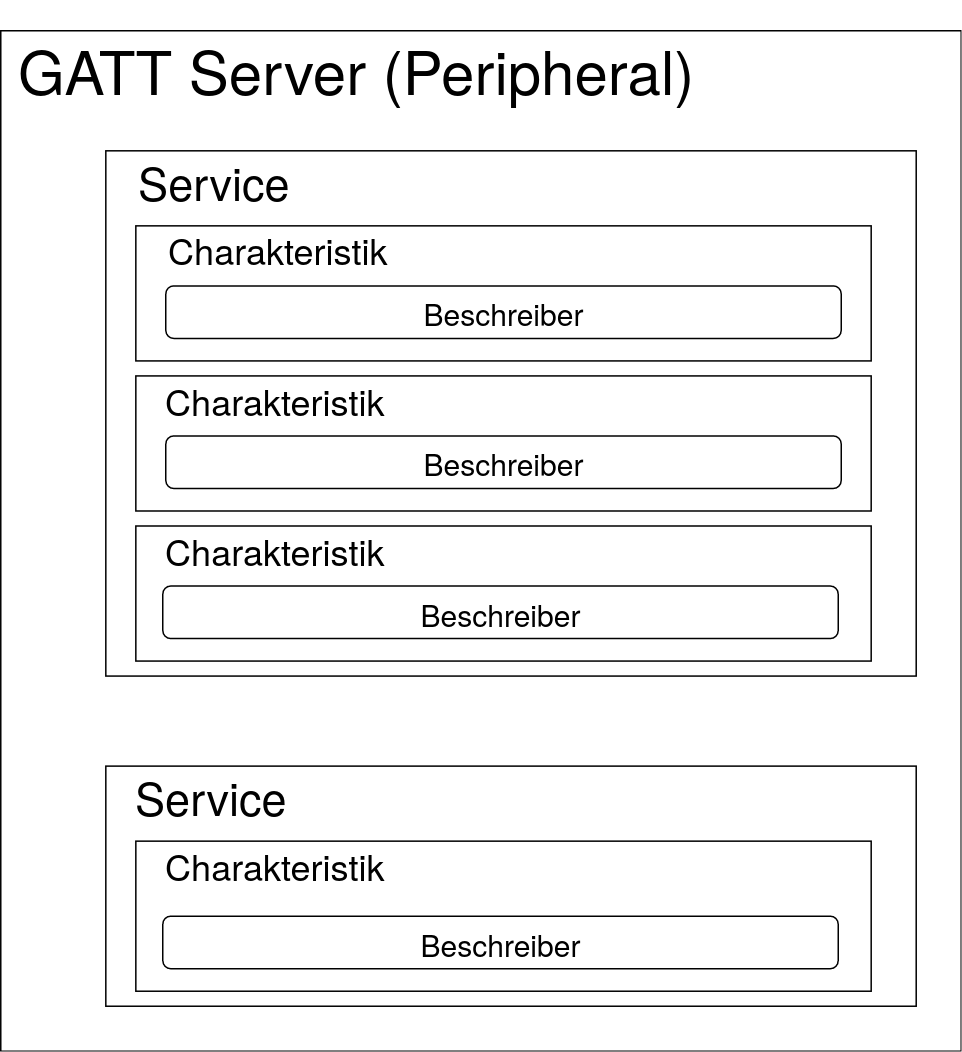
\includegraphics[width=0.75\linewidth]{\figdir/GATT}
	\caption{Aufbau eines \ac{gatt} Servers \cite[Seite 57]{Townsend14:GSB}}
	\label{FIG:gatt}
\end{figure}

\noindent In Abbildung \ref{FIG:gatt} ist ein \ac{gatt} Server abgebildet. Man kann hier verschiedene Ebenen erkennen. Jeder Server kann über einen oder mehrere Services verfügen. Diese wieder können eine oder mehrere Charakteristiken enthalten. Jeder Service ist so konfiguriert, dass mit ihm eine bestimmte Aufgabe erfüllt werden kann. So kann ein Service beispielsweise dafür gedacht sein, sämtliche Funktionen bereitzustellen um Daten an den Server zu schreiben. Ein anderer Service wiederum kann dann für sämtliche Lesezugriffe gedacht sein \cite[Seite 32]{Usama17:BBS}. Die Charakteristiken, welche jeder Service enthält enthalten dann mindestens zwei Attribute. Zum Einen ein Leseattribut, welches Informationen über die Charakteristik, wie unter anderem den "`Handle"', die \ac{uuid} und die Eigenschaften enthält. Zum Anderen den eigentlichen Wert, den die Charakteristik enthält. Die Charakteristikeigenschaft sagt dabei aus, um welche Art es sich bei ihr handelt. Folgende Möglichkeiten stehen unter anderem zur Auswahl: 
\begin{itemize}
	\item{Broadcast}
	\item{Lesen}
	\item{Schreiben ohne Antwort}
	\item{Schreiben}
	\item{Benachrichtigen}
	\item{...}
\end{itemize} 
Mit diesem Wissen über eine Charakteristik weis ein Client, welche Aktion er mit dieser ausführen kann. Der Beschreiber, der im Kern jeder Charakteristik zu finden ist liefert zusätzliche Informationen zur Charakteristik. Sie bestehen immer aus einem einzigen Attribut. Dabei kann es sich beispielsweise um einen String handeln, der eine Beschreibung liefert, welche Funktion die Charakteristik ausübt \cite[Seite 59ff]{Townsend14:GSB}.\\ 

\subsection{Kommunikation}
\label{ss:funktionsweise:kommunkation}

Nachdem in Kapitel \ref{ss:funktionsweise:protokollstack} der allgemeine Aufbau von \ac{ble} erläutert wurde, wird im nachfolgenden Kapitel auf das Kernelement, die tatsächliche Kommunikation zwischen zwei oder mehreren Geräten, von \ac{ble} eingegangen. Dabei werden drei Elemente im besonderen betrachtet. Die Bekanntmachung, die Verbindung und den Datenaustausch.\\

\subsubsection{Advertisement}
\label{sss:funktionsweise:advertisement}

Das "`Advertsement"' oder zu deutsch die Bekanntmachung ist die Funktion, mittels welcher sich Geräte, die Bereit sind sich zu koppeln bei suchenden Geräten bekanntmachen. Allerdings kann die Bekanntmachung auch für einen "`Broadcast"' von Daten ohne explizites Zielgerät verwendet werden.\\

\noindent Für das "`Advertisement"' sind drei der 40 Kanäle, in die der Frequenzbereich auf dem \ac{ism} Band unterteilt ist, reserviert. Ein Gerät kann diese Kanäle nutzen und ein Paket senden, welches verbindungsspezifische Daten bereitstellt. Generell gibt es folgende vier unterschiedliche Pakete, welche somit gesendet werden können:
\begin{itemize}
	\item{ADV\_IND}
	\item{ADV\_DIRECT\_IND}
	\item{ADV\_SCAN\_IND}
	\item{ADV\_NONCONN\_IND}
\end{itemize} 
Das "`ADV\_IND"' Paket sendet eine Bekanntmachung an alle Geräte, die zuhören und gibt bekannt, dass das Gerät bereit ist sich mit jeglichem Gerät zu verbinden. Im Gegensatz dazu sendet das "`ADV\_DIRECT\_IND"' Paket eine direkte Nachricht an ein bestimmtes Gerät, dass es bereit ist, sich mit genau diesem zu koppeln. Um das zu gewährleisten enthält die "`Payload"' des Paketes die beiden \ac{ble} Adressen der betroffenen Geräte. Diese beiden Pakete lassen auch zu, dass sich die Geräte miteinander verbinden. Die restlichen zwei Pakete lassen dies wiederum nicht zu. So ermöglicht das "`ADV\_SCAN\_IND"' Paket lediglich einen "`Broadcast"' an alle hörenden Geräte zu senden, dass dieses Gerät in Reichweite ist. Es ist als sichtbar für die anderen Geräte. Um jedoch eine Verbindung einzugehen müssen weitere Schritte unternommen werden. Das letzte Paket teilt allen Geräten in Reichweite mit, dass dieses Gerät nicht für eine Kopplung zu Verfügung steht. Alle Pakete bis auf das "`ADV\_DIRECT\_IND"' Paket können zusätzlich Daten enthalten, die über das "`Advertisement"' hinausgehen. Das ermöglicht auch den Einsatz von \ac{ble} Beacons, welche ohne eine Verbindung einzugehen Daten an alle Geräte in Reichweite senden können. \cite{ADV:WWW}.\\
  Sollte das "`Peripheral"' diese akzeptieren
\subsubsection{Verbindung}
\label{sss:funktionsweise:verbindung}

Nachdem in Kapitel \ref{sss:funktionsweise:linked} erklärt wurde, wie Pakete aufgebaut sind und übertragen werden, gilt es noch zu erläutern, wie eine Verbindung in \ac{ble} abläuft, um diese Pakete tatsächlich transferieren zu können. Nachdem ein "`Central"' ein Gerät über das "`Advertisement"' gefunden hat, kann es eine Verbindungsanfrage initiieren. In diesem Paket sind drei wichtige Verbindungsparameter angegeben:
\begin{itemize}
	\item{Verbindungsintervall}
	\item{"`Slave"' Latenz}
	\item{Überwachungszeitüberschreitung}
\end{itemize}
Das Verbindungsintervall legt die Zeit fest, die zwischen zwei Verbindungsevents verstreicht. Eine Verbindung in \ac{ble} besteht ausschließlich aus derartigen Ereignissen und bleibt solange bestehen, wie diese regelmäßig stattfinden. Bei diesem Intervall gilt es abzuwägen, was wichtiger ist. Je geringer dieses Intervall ist, desto schneller ist die Verbindung. Jedoch verbraucht dieses Verhalten auch mehr Energie. Das "`Central"' muss also im Vorhinein festlegen, was für die kommende Verbindung wichtiger ist \cite{CON:WWW}. Die "`Slave"' Latenz legt die Nummer der Verbindungsevents an, die der "`Slave"' erlaubt ist zu überspringen, bevor die Verbindung als beendet gilt. Ein weiterer Weg, wie eine Verbindung vorzeitig abgebrochen werden kann, wird durch die Überwachungszeitüberschreitung festgelegt. Bei dieser wird definiert, wie viel Zeit zwischen zwei erfolgreichen Übertragungen verstreichen darf. Sollte es also zu dem Fall kommen, dass über einen längeren Zeitraum erfolglos Pakete versendet werden, wird die Verbindung beendet \cite[Seite 23]{Townsend14:GSB}.\\

\begin{figure}[h]
	\centering
	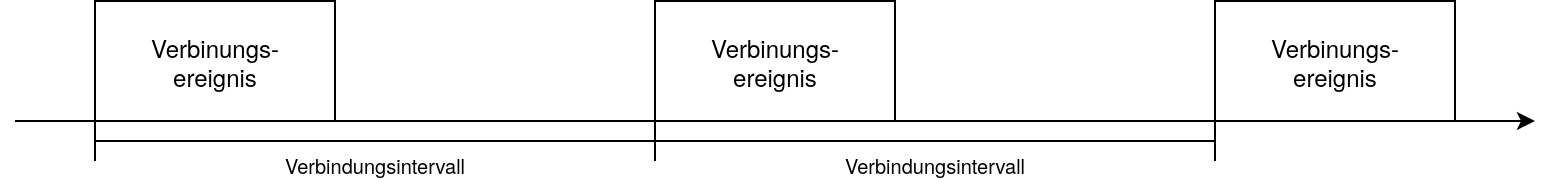
\includegraphics[width=\linewidth]{\figdir/ConEv}
	\caption{Ablauf einer \ac{ble} Verbindung \cite{CON:WWW}}
	\label{FIG:conenv}
\end{figure}

\noindent Wenn das "`Peripheral"' die Verbindung annimmt, wird diese, wie in Abbildung \ref{FIG:conenv} dargestellt, aufgenommen. Jedes dieser Ereignisse folgt einem bestimmten Ablauf. Zuerst überträgt der "`Master"' eine Anfrage an den "`Slave"'. Dieser empfängt die Anfrage und verarbeitet diese. Anschließende sendet er eine entsprechende Antwort, die der "`Master"' empfängt. Wichtig dabei ist, das der "`Master"' nicht nur die Verbindung initiiert, sondern auch sämtliche Anfragen. Nachdem das definierte Verbindungsintervall abgelaufen ist, wird das nächste Verbindungsevent gestartet \cite{CON:WWW}.\\       

\section{Anwendungsbeispiel iBeacon}
\label{s:ibeacon}

Lorem Ipsum

\subsection{Funktionsweise}
\label{ss:ibeacon:funktionsweise}

Lorem Ipsum

\subsection{Kommunikation}
\label{ss:ibeacon:kommunikation}

Lorem Ipsum

\section{Vergleich mit anderen Kommunikationsprotokollen}
\label{s:vergleich}

Nachdem in den vorherigen Kapiteln ausführlich auf die Funktionsweise und die resultierenden Vorteile von \ac{ble} eingegangen wurde, widmet sich dieses Kapitel dem Vergleich mit anderen bekannten Protokollen aus dem Bereich der \ac{iot}. Besonders hervorgehoben werden dabei die Vorteile und Nachteile gegenüber diesen Protokollen. Um eine vernünftige Auswahl an Protokollen treffen zu können betrachten wir in diesem Zusammenhang den Protokollumfang, welchen die "`Amazon Echo"' mit sich bringt um im Jahr 2019 sämtliche Funktionen für eine "`Smarthome"' Integration zu erreichen. Zusätzlich wird eine weitere Technologie betrachtet, welche hauptsächlich im freien zur Anwendung kommt.\\  

\subsection{ZigBee}
\label{ss:vergleich:zigbee}

Dieses Protokoll ist wie die meisten \ac{iot} Protokolle darauf ausgelegt möglichst wenig Energie zu verbrauchen. Es ist hauptsächlich für die Steuerung von Geräten wie beispielsweise Rollosteuerungen oder Lampen gedacht. "`Zigbee"' selbst verfügt aus Energiegründen über keine große Reichweite. Es kann dennoch ein komplettes Haus abdecken. Das liegt daran, dass dieses Protokoll ein Netzwerk mit verschiedenen "`Zigbee"' Geräten aufspannt. So kommuniziert die "`Amazon Alexa"' ausschließlich mit dem ersten Gerät des Netzwerkes. Die Information wird dann durch das Netzwerk gereicht und an das Zielgerät übermittelt. Dieses kann dann die gewünschte Aktion ausführen. In einem derartigen Netzwerk gibt es drei Instanzen. Zuallererst den Koordinator, der das Netzwerk startet und steuert. Jeder Teilnehmer, der kein Endknoten ist, nimmt die Rolle eines Routers an. Dieser gibt Nachrichten, die nicht an ihn gerichtet sind, weiter. Die letzte Instanz ist dann der Endknoten. Dieses Netzwerkkonstrukt hat jedoch zur Folge, dass der Einsatzort von "`Zigbee"' nur stationär möglich ist.\\

\noindent Sollte man ein Gerät aus dem Netzwerk entfernen ist dieses dazu in der Lage die entfernte Route zu erkennen und eine Umleitung zu Geräten einzurichten, die sonst verloren werden würden. Um ein Gerät in das Netzwerk einzufügen muss man lediglich mit Hilfe des Koordinators einen Kanalscan ausführen. Dieser erkennt das Gerät, welches man mittels Nutzerinteraktion für 180 Sekunden sichtbar machen kann, und fügt dieses in das Netzwerk ein. Das Hinzufügen eines Gerätes ist also ähnlich einfach wie im \ac{ble} Standard \cite{ZA:Zig}.\\

\noindent "`Zigbee"' ist ein Protokoll welches perfekt für die Fernsteuerung von Geräten wie Lichter, Steckdosen, oder Motorsteuerungen ist. Dafür benötigt es weniger Energie als \ac{ble}, da es seine Reichweite über ein Netzwerk erreicht. Zusätzlich sendet es kleinere Pakete, was wiederum Energie einspart. Allerdings ist es aufgrund des Netzwerkes auch an einen bestimmten Ort gebunden, wohingegen \ac{ble} nicht ortsgebunden ist. Durch die größeren Datenpakete ermöglicht \ac{ble} auch den Austausch größerer Datenmengen und bietet somit einen größeren Funktionsumfang.\\

\subsection{Wlan}
\label{ss:vergleich:wifi}

Im Gegensatz zu \ac{ble} ist "`Wlan"' kein \ac{iot} Netzwerkprotokoll. Um dieses Protokoll zu betreiben benötigt man einen Router, welcher die verschieden Endgeräte miteinander verbindet. "`Wlan"' verfügt zwar über einen "`Ad-Hoc"' Modus, bei welchem sich Geräte direkt miteinander verbinden können. Dabei ist der Aufbau allerdings aufwändiger als bei \ac{ble}, da der Host manuell eine IP Adresse konfigurieren muss. Zusätzlich hat man in diesem Modus keinen Zugriff auf das Internet. Dieser Modus ist zwar sehr ähnlich einsetzbar wie \ac{ble}, benötigt allerdings viel mehr Energie, da der "`Wlan"' Standard größere Paketgrößen definiert. Dies wiederum bietet den Vorteil, dass eine schnellere Kommunikation möglich ist.\\

\noindent Normalerweise wird "`Wlan"' im Infrastrukturmodus"' in Verbindung mit einem Router und Zugang zum Internet betrieben. Das bietet den Vorteil, dass die Reichweite von "`Wlan"' beinahe unbegrenzt ist. Im Zusammenhang mit dem "`Smarthome"' kann man so beispielsweise sein Zuhause überwachen, wenn man an einem gänzlich anderen Ort ist \cite{MUE:Wlan}.\\

\noindent "`Wlan"' bietet einige Vorteile gegenüber \ac{ble}. Darunter sind ganz klar die Reichweite und die schnellere Übertragung von größeren Daten. Diese haben allerdings den Nachteil, dass sie an Infrastruktur gebunden sind, die nicht überall verfügbar ist. Auch der dadurch erhöhte Energieverbrauch stellt ein Problem dar. \ac{ble} hingegen benötigt keine Infrastruktur und ist überall verfügbar, wo man ein Gerät einsetzen möchte.\\ 

\subsection{LoRaWAN}
\label{ss:vergleich:lora}

"`LoRaWAN"' ist ein Netzwerk, welches nicht im "`Smarthome"' zum Einsatz kommt. Die Kernaufgabe stellt es dar, eine möglichst große Reichweite abzudecken. Dabei können bis zu 15 Kilometer mit einem Sendemast abgedeckt werden. Dies ist möglich, da sehr kleine Pakete versendet werden und daher eine Frequenz verwendet werden kann, die eine hohe Reichweite aufweist, jedoch im Datenfassungsvermögen eingeschränkt ist.\\

\noindent Für dieses Protokoll benötigt man allerdings Infrastruktur. Es wird ein Netzwerkserver benötigt, der mit einem oder mehreren Gateways verbunden ist. Diese sind mit einer Antenne ausgestattet und kommunizieren mit den "`LoRa"' Sensoren \cite{LO:WWW}.\\

\noindent Die beiden Protokolle \ac{ble} und "`LoRaWAN"' stellen also das genaue Gegenteil voneinander dar. Wohingegen \ac{ble} eine geringe Reichweite aufweist, allerdings keine Infrastruktur benötigt und eine moderate Datenrate besitzt, kann "`LoRaWAN"' ein riesiges Gebiet abdecken. Dabei muss dieses allerdings in sämtlichen anderen Bereichen große Abstriche machen. Die einzige Gemeinsamkeit, welche beide Protokolle aufweisen ist der Geringe Energieverbrauch.\\ 

\section{Fazit}
\label{s:fazit}

Lorem Ipsum
%%% Local Variables: 
%%% mode: latex
%%% TeX-master: "thesis.tex"
%%% End: 
